\section{Types of SQL Commands}
\paragraph{} There are five different sub-languages \acs{SQL}: \acs{DCL}, \acs{DDL}, \acs{DML}, \acs{DQL} and \acs{TCL}.
\begin{center}
	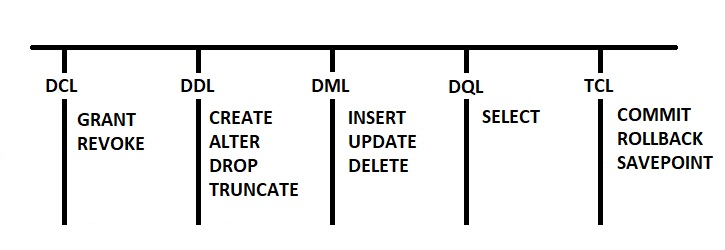
\includegraphics[scale=0.8]{types-of-sql-commands}
\end{center}
\paragraph{} \textbf{\acf{DCL}}
\begin{itemize}
	\item Is responsible for administrative tasks, mainly granting and revoking user privileges.
	\item \textbf{\acs{DCL} commands:}
	\subitem GRANT/REVOKE/FLUSH PRIVILEGES, SHOW GRANTS.
	\item \textbf{Non \acs{DCL} commands} covered in this section as they are related to \acs{DB} users and roles:
	\subitem CREATE/RENAME/DROP USER.
	\subitem CREATE/RENAME/DROP/SET DEFAULT ROLE.
\end{itemize}
\paragraph{} \textbf{\acf{DDL}}
\begin{itemize}
	\item Is responsible for defining the structure of the data.
	\item \textbf{Important:} \acs{DDL} commands are auto-committed, once executed changes are permanently saved in the database. Rollback is not possible.
	\item \textbf{\acs{DDL} commands:}
	\subitem CREATE/ALTER/DROP/TRUNCATE/COMMENT/RENAME TABLE.
	\subitem CREATE/DROP VIEW.
	\subitem CREATE/DROP/SHOW/USE DATABASE.
\end{itemize}
\paragraph{} \textbf{\acf{DML}}
\begin{itemize}
	\item Is responsible for creating, updating and deleting data.
	\item From \acs{CRUD} operations it is responsible for: Create, Update and Delete operations.
	\item \textbf{\acs{DML} commands:}
	\subitem INSERT/UPDATE/MERGE/DELETE.
\end{itemize}
\paragraph{} \textbf{\acf{DQL}}
\begin{itemize}
	\item Is responsible for reading/querying data from the database.
	\item From \acs{CRUD} operations it is responsible for: Read operation.
	\item \textbf{\acs{DQL} commands:}
	\subitem SELECT.
\end{itemize}
\paragraph{} \textbf{\acf{TCL}}
\begin{itemize}
	\item Is responsible for controlling transaction behavior.
	\item \acs{TCL} commands $\underline{can}$ only be used with \acs{DML} and \acs{DQL} commands.
	\item \acs{TCL} commands $\underline{cannot}$ be used with \acs{DCL} or \acs{DDL} commands as they are auto-committed.
	\item \textbf{\acs{TCL} commands:}
	\subitem START TRANSACTION/COMMIT/ROLLBACK.
	\subitem SAVEPOINT/ROLLBACK TO SAVEPOINT.
	\subitem START TRANSACTION READ WRITE/READ ONLY.
	\subitem SET TRANSACTION ISOLATION LEVEL.
	\subsubitem SERIALIZABLE/READ COMMITTED/UNCOMMITTED/REPEATABLE.
\end{itemize}